\section{Druckvorgang}
%\todoinline{Beschreibung, warum die Bauteile auf- und verteilt werden müssen}
%genaue Maße der Druckplatte; siehe: 
%\verb|https://eu.makerbot.com/fileadmin/Inhalte/Support/Manuals/German_UserManual_V.4_Replicator2.pdf|
%oder Kapitel 4 unten
% [28.5 x 15.3 x 15.5 cm]
Nachdem die einzelnen Bestandteile des Modells berechnet wurden, können diese gedruckt werden.
Hierbei ist allerdings zu bedenken, dass alle einzelnen Bauteile nicht in einem Druckvorgang gedruckt werden können, da die Grundfläche des 3D-Druckers begrenzt ist. \\
In unserem Fall wies diese eine Länge von 28,5 cm und eine Breite von 15,2 cm auf (vgl. Quelle \cite{makerbotspecs}).

\subsection{Minimierung der Druckvorgänge}
Um die Dimensionen der Grundfläche effektiv auszunutzen, werden einzelne Elemente des Modells nach der Größe sortiert und dann solange nebeneinander angeordnet, bis die Breite der Druckfläche mit dem nächsten Element überschritten werden würde.
Anschließend wird eine neue Reihe eröffnet, in der nun neue Elemente platziert werden. 
Dieser Prozess wird solange fortgeführt, bis die Länge der Druckfläche überschritten werden würde. \\
Dann wird eine neue Gruppierung von Objekten bzw. \icode{Union} erstellt, in welcher der Algorithmus weiterläuft.
Das Resultat zeigt eine Liste von Objekten, die eine platzeffiziente Anordnung dieser repräsentiert.
Die Vereinigungen von Grundplatten werden zusätzlich um 180$^\circ$ gedreht, damit keine Überhänge in der Datei vorkommen, was zu einer Verlängerung der Druckzeit führen würde.\\
Jedes einzelne Element in der Liste kann mit einem Durchgang gedruckt werden(vgl. Abb.~ \thebildnrnext, 23 und 24).

\begin{Bild}{platzeffiziente Platzierung von Wänden (Screenshot der Verfasser)}
	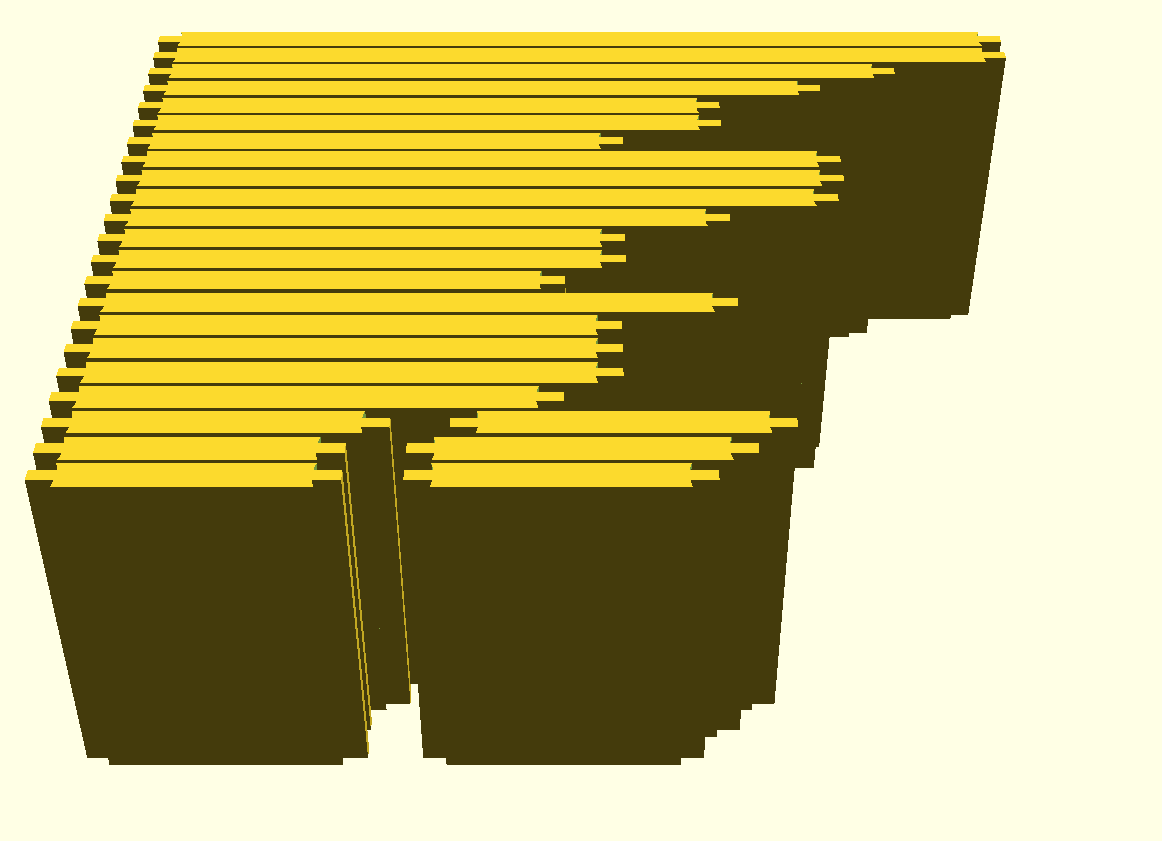
\includegraphics[width = 110mm]{Bilder/WallPlacement}
\end{Bild}

\begin{Bild}{platzeffiziente Anordnung von Eckpfeilern auf der Grundfläche (rot) (Abbildung der Verfasser)}
	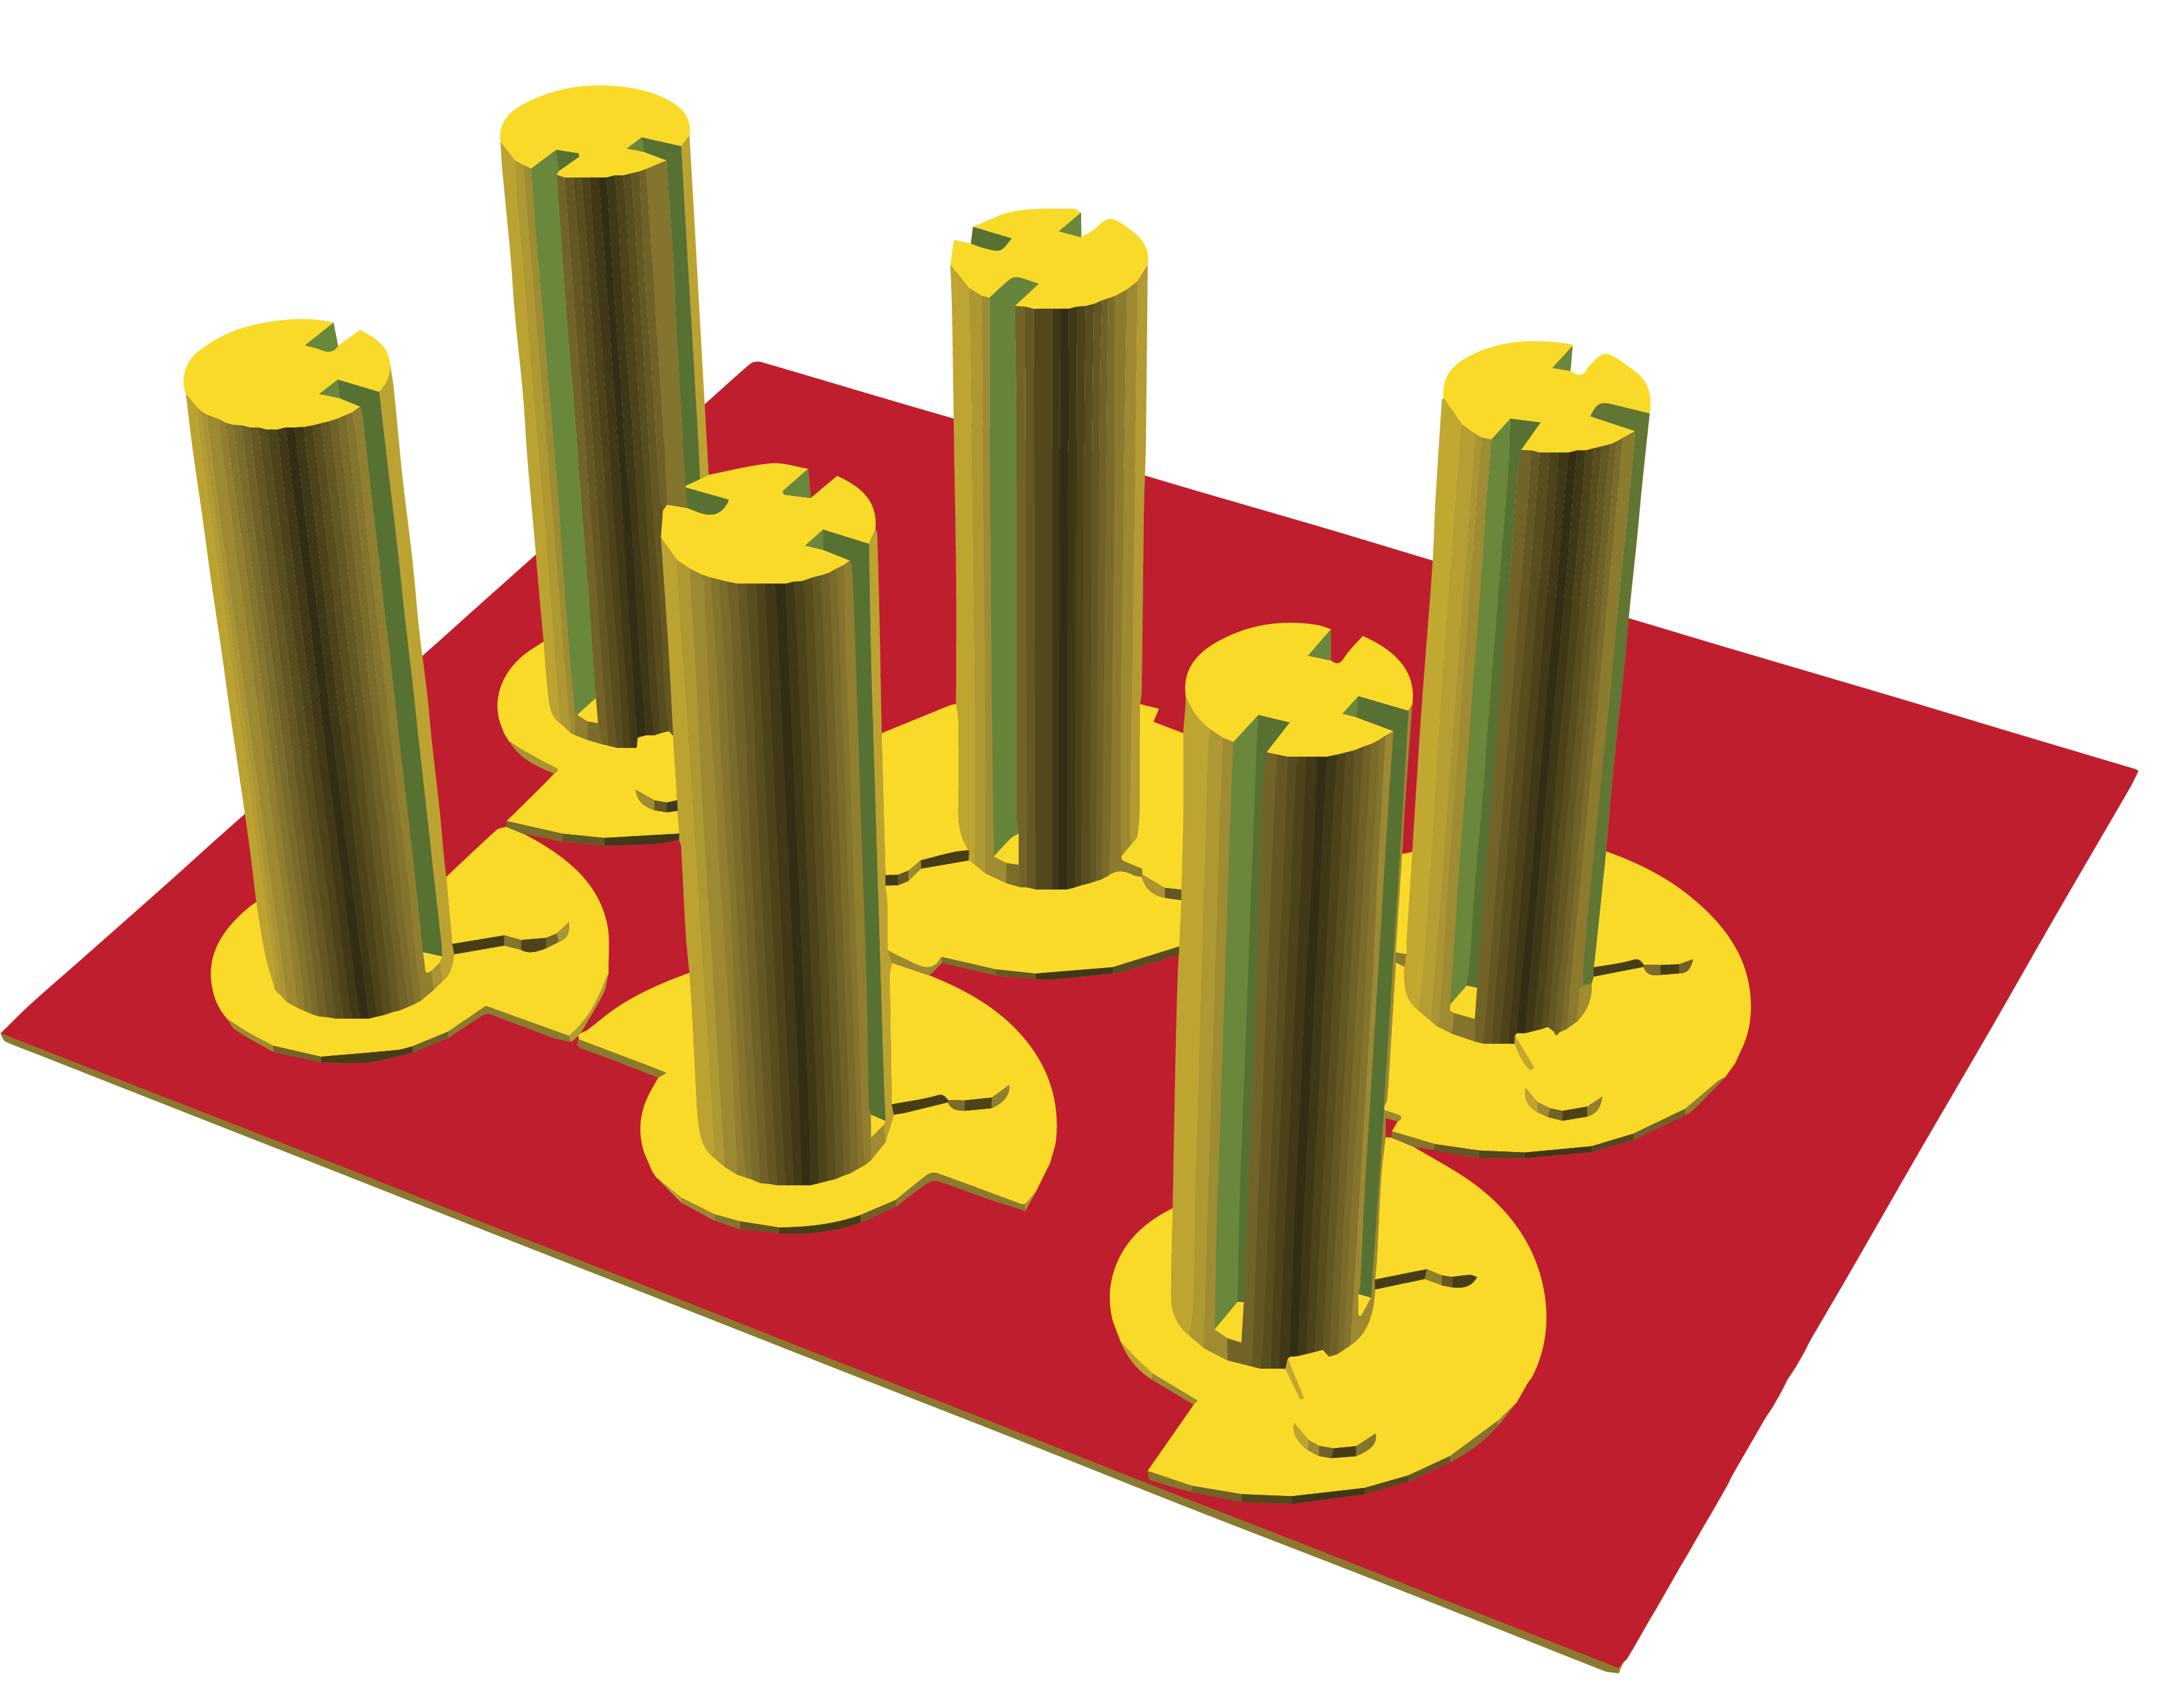
\includegraphics[width = 110mm]{Bilder/PlacementCorners-12}
	\label{corner}
\end{Bild}

\begin{Bild}{platzeffiziente Anordnung von Grundplatten auf der Grundfläche (rot) (Abbildung der Verfasser)}
	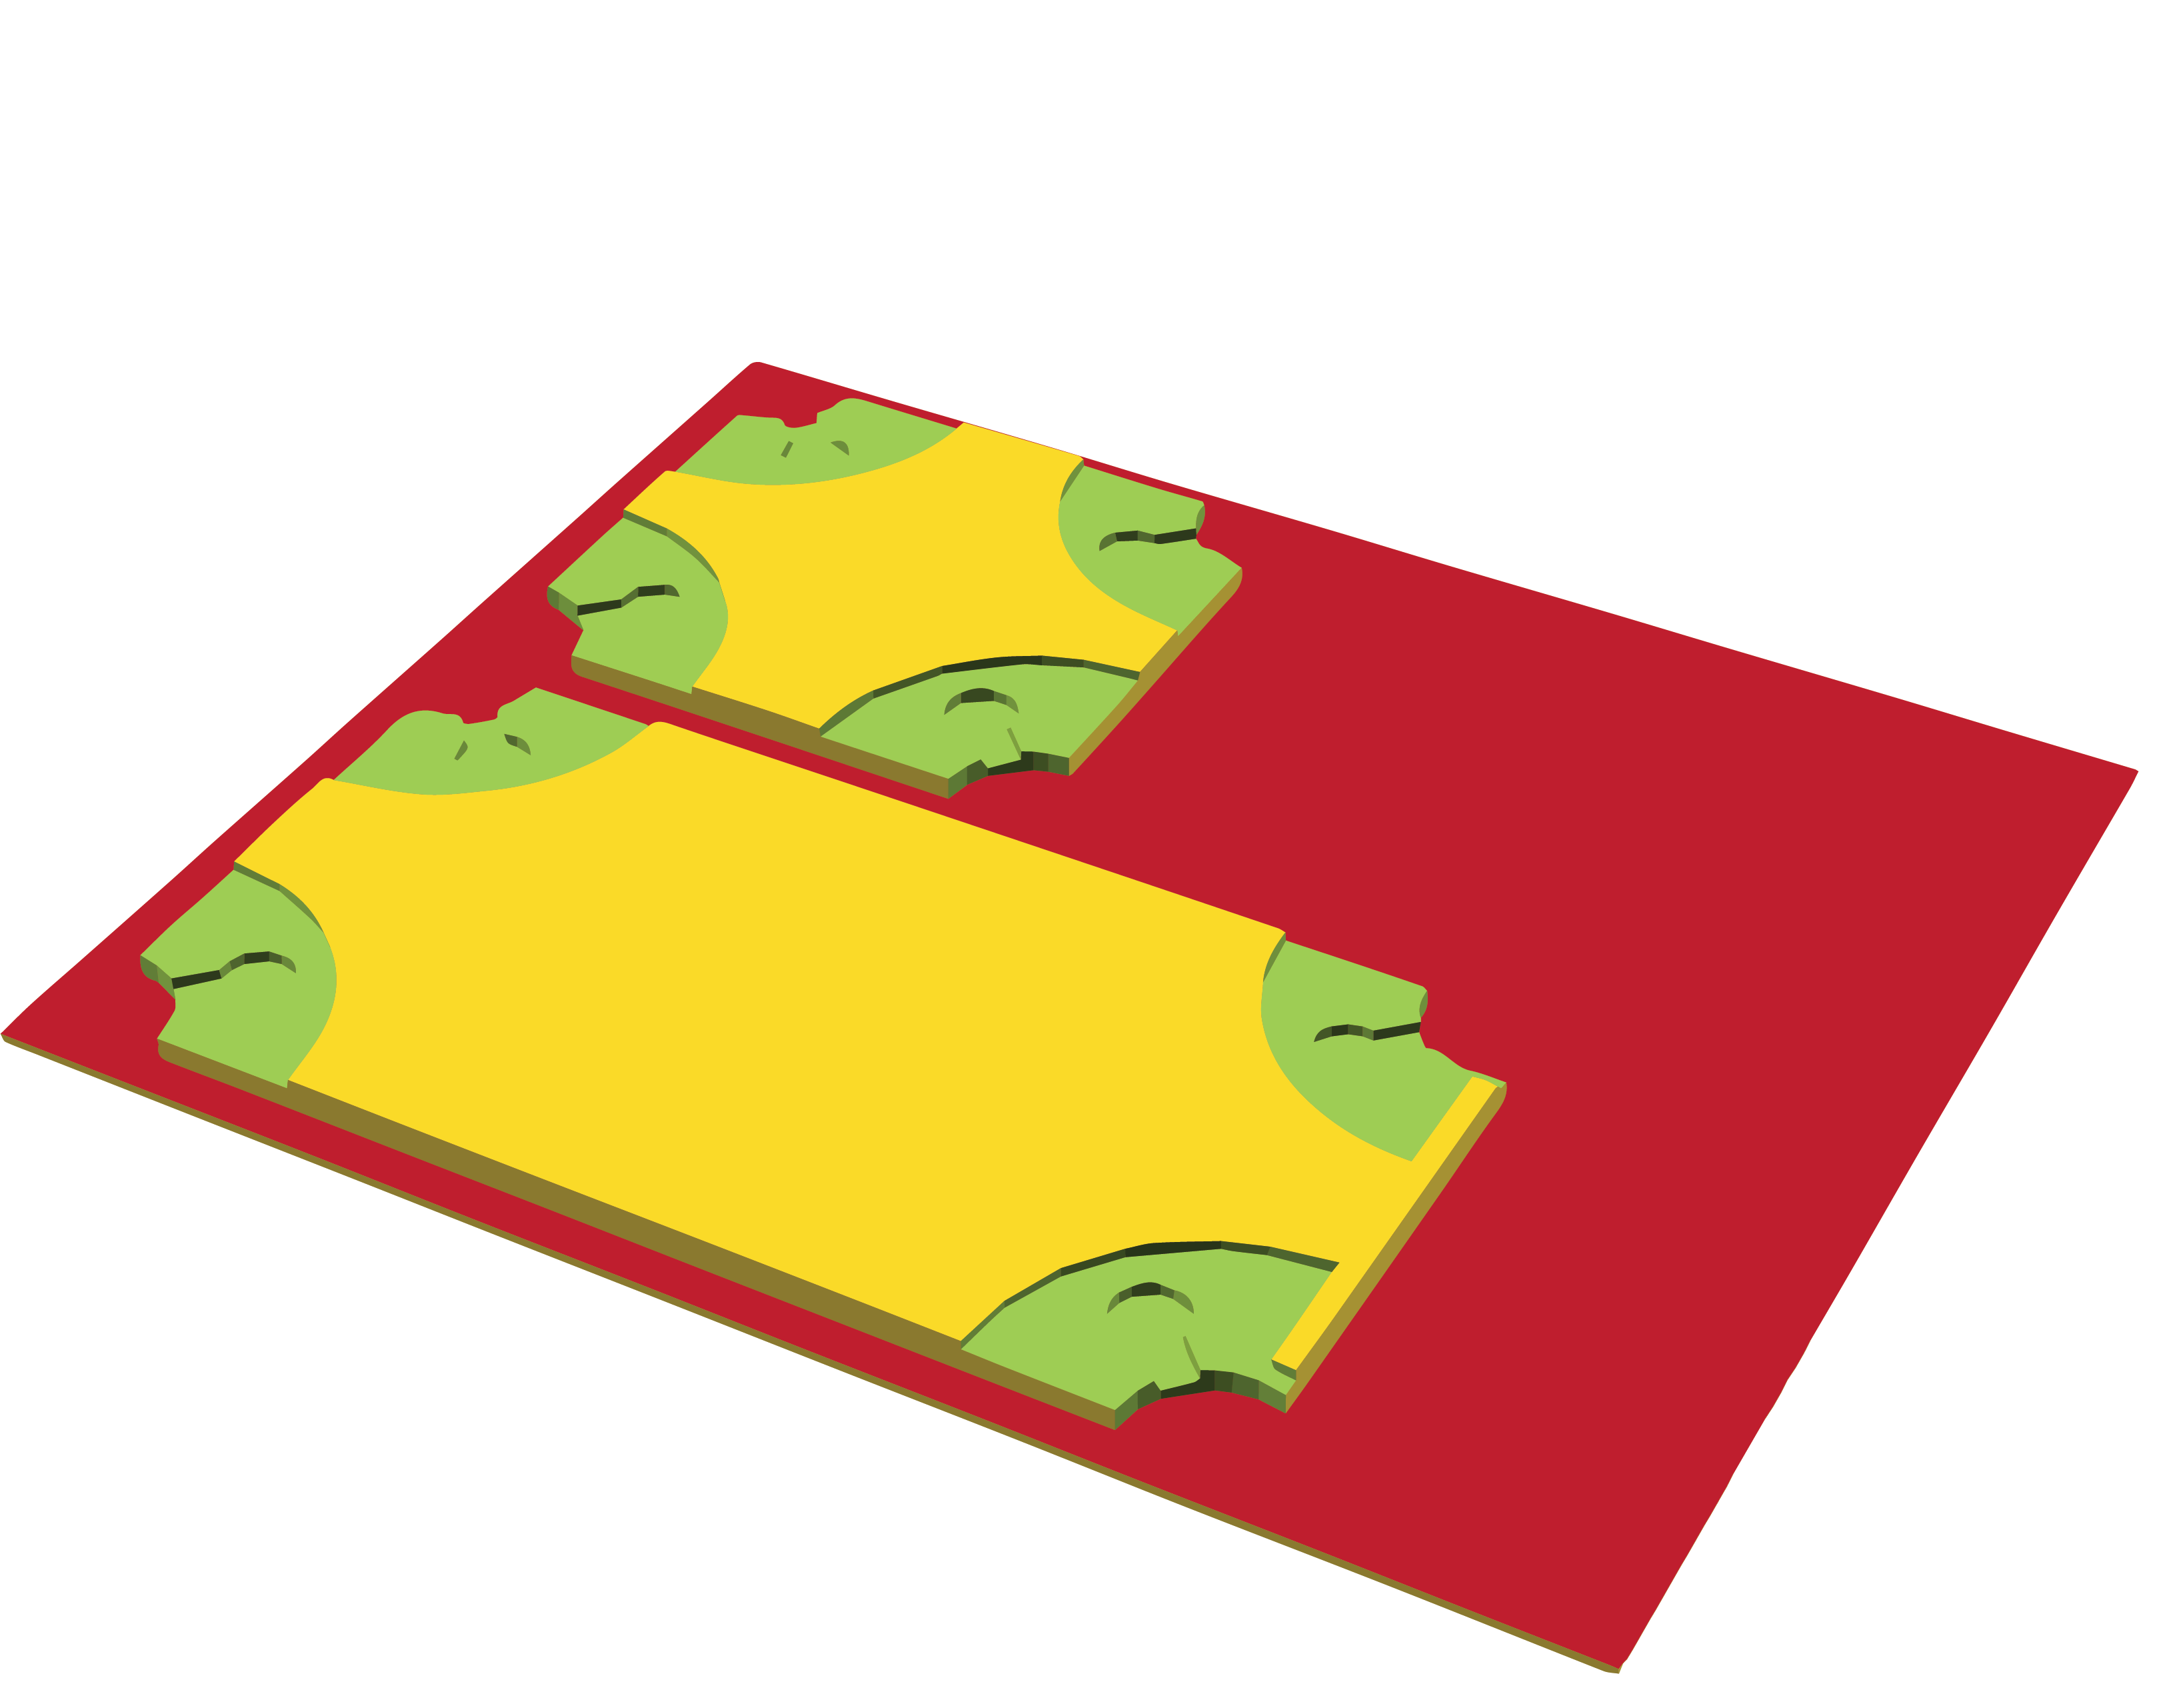
\includegraphics[width = 110mm]{Bilder/PlacementBasePlate-13}
\end{Bild}

\subsection{Ermittlung der Größen}
Das Einzige, was die Strukturen Wand- und Eckteil, sowie Grundplatte in dem beschriebenen Algorithmus voneinander unterscheidet, ist die Größe, welche unterschiedlich bestimmt wird.
Da die Anordnung ein zweidimensionales Problem ist, wird die Höhe der Objekte nicht berücksichtigt.

\subsubsection{Wände}
Die Wandelemente werden durch eine Kante dargestellt und so modifiziert, dass sie in die Eckpfeiler gesteckt werden können.
Als Länge wird die Länge der zugehörigen Kante verwendet.
Die Breite ermittelt sich durch die definierte \icode{wallWidth} der übergebenen \icode{Params}-Klasse.

\subsubsection{Eckpfeiler}
Für die Größenberechnung der Eckpfeiler wird der längste Eckpin ermittelt, welcher an dem jeweiligen Objekt anliegt.
Die Länge dieses Eckpins stellt dann die Seitenlänge eines Quadrats dar, welche die Ausmaße des Eckpfeilers angibt.

\subsubsection{Grundplatten}
Um die optimale Größe der Grundplatten zu berechnen, wird die OMBB dieser berechnet.
Für die Berechnung wird zuerst die konvexen Hülle ermittelt, da nach dem von Freeman und Shapira bewiesenen Satz, eine Seite des minimalen Begrenzungsrechtecks kollinear mit einer der konvexen Hülle sein muss (vgl. Quelle \cite{ombb}).
Für die Ermittlung wird der \q{Gift Wrapping Algorithm} herangezogen.
Bei diesem Algorithmus wird zuerst der Punkt mit der kleinsten Ordinate als Startpunkt $P_0$ festgelegt.
Gibt es mehrere dieser Punkte, wird aus denen der Punkt mit der kleinsten Abszisse gewählt.
Von $P_0$ ausgehend wird eine Gerade durch einen beliebigen Punkt $P$ des Polygons gelegt und anschließend überprüft, ob es einen Punkt $S$ gibt, der links der Geraden liegt.
Im Programm geschieht das durch die Berechnung des Winkels zwischen den Vektoren $\overrightarrow{{P_0}P}$ und $\overrightarrow{{P_0}S}$ mithilfe der \icode{Vector.angleTo(Vector v)} Methode.
Ist dieser Winkel kleiner gleich $180^\circ$, liegt $S$ links von der Gerade durch $P_0$ und $P$.
$S$ wird folglich als neuer Punkt $P$ gesetzt und die Berechnung fortgesetzt.
Der Vorgang wird solange durchgeführt, bis alle Punkte überprüft wurden und ein nächster Punkt $P_1$ der konvexen Hülle feststeht.
Der Algorithmus wird nun fortgeführt mit $P_1$ als Ausgangspunkt, bis der Anfangspunkt $P_0$ wieder erreicht wurde, sodass die konvexe Hülle \q{geschlossen} ist.\\
Nun wird die konvexe Hülle fortlaufend rotiert, so dass eine Seite parallel zur x-Achse ist.
Dadurch kann man das Begrenzungsrechteck durch Feststellen der Extremwerte des rotierten Polygons ermitteln.
Der Flächeninhalt des Rechtecks aus den Punkten $A(x_{min}, y_{min})$, $B(x_{min}, y_{max})$, $C(y_{max}, x_{max})$ und $D(x_{max}, y_{min})$ wird gespeichert.
Der Algorithmus wiederholt diese Abfolge für jede Seite, bis alle Seiten der konvexen Hülle behandelt wurden. %Gerade ist thematisch falsch
Als Ergebnis erhält das Programm die Breite, Höhe der OMBB und den nötigen Winkel, mit welchem diese erreicht wird.\\
Diese Werte werden auf die Grundplatte angewendet, wobei die Breite und Höhe jeweils vergrößert wird, damit die Modifikationen berücksichtigt werden, die an der Grundplatte durchgeführt wurden (vgl.~\ref{gr}).